\documentclass[11pt, a4paper]{article}
\usepackage{geometry}
\geometry{left=2cm, right=2cm, top=2cm, bottom=2cm}
\usepackage{amsmath} % For math
\usepackage{graphicx} % For images if needed
\usepackage{siunitx} % For units
\usepackage{array}
\usepackage[utf8]{inputenc}
\usepackage[T1]{fontenc}
\usepackage{hyperref}

\title{Year 11 Physics - Worksheet 2 \\ Thermodynamics: Quantifying Heat & Phase Change}
\date{Module 3}
\author{Student Name: \underline{\hspace{5cm}} ID: \underline{\hspace{3cm}}} % Placeholder for student info

\begin{document}
\maketitle

\section*{Part 1: Heating Curve Analysis (Knowledge Node N5 Analyse)}

1.  The graph below shows a typical heating curve for water, starting as ice below 0\si{\celsius} and ending as steam above 100\si{\celsius}. Energy is added at a constant rate.

    \begin{center}
    % Placeholder for graph - ideally insert an image or tikzpicture here
    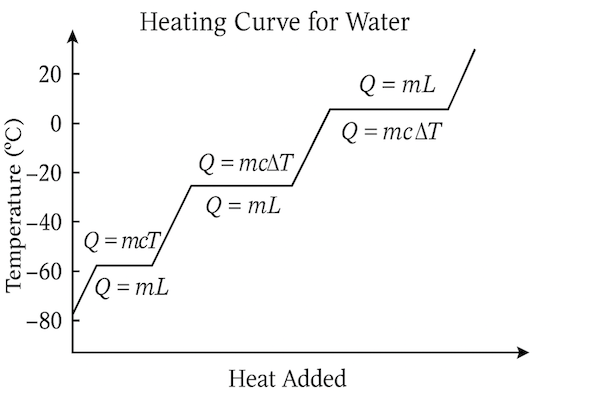
\includegraphics[width=0.4\textwidth]{img/water_heating.png}
    \end{center}

    \begin{itemize}
        \item[(a)] On the graph above, clearly \textbf{label} the 5 sections corresponding to: Heating Ice, Melting Ice, Heating Water, Boiling Water, Heating Steam.
        \item[(b)] In which section(s) is the added energy increasing the *kinetic energy* of the particles the most? \textbf{Explain} your reasoning. \vspace{1cm}
        \item[(c)] In which section(s) is the added energy primarily increasing the *potential energy* (overcoming bonds) of the particles? \textbf{Explain} your reasoning. [Literacy N5] \vspace{1cm}
        \item[(d)] Indicate on the graph where the formula Q=mcΔT would be used to calculate energy added, and where Q=mL would be used.
    \end{itemize}
    \textit{[Numeracy Focus: Graph interpretation - N5]}

2.  \textbf{Define} the following terms:
    \begin{itemize}
        \item Specific Heat Capacity (c): \vspace{1cm}
        \item Latent Heat of Fusion (Lf): \vspace{1cm}
        \item Latent Heat of Vaporization (Lv): \vspace{1cm}
    \end{itemize}
    [Literacy N3, N5]

\section*{Part 2: Calculations (Knowledge Nodes N3 Apply, N5 Apply)}
\textit{(Use the provided data table for c and L values)}

\textbf{Worked Example 1 (Q=mcΔT):} Calculate heat needed to warm 200g (0.2kg) water from 20\si{\celsius} to 50\si{\celsius}. ($c_{water} = 4186 \, \si{J.kg^{-1}.K^{-1}}$)
$Q = mc\Delta T = (0.2\,\si{kg})(4186\,\si{J.kg^{-1}.K^{-1}})(50-20\,\si{K}) = 25116\,\si{J}$

\textbf{Worked Example 2 (Q=mL):} Calculate heat needed to melt 50g (0.05kg) of ice at 0\si{\celsius}. ($L_{f, water} = 3.34 \times 10^5 \, \si{J.kg^{-1}}$)
$Q = mL_f = (0.05\,\si{kg})(3.34 \times 10^5\,\si{J.kg^{-1}}) = 16700\,\si{J}$

\textbf{Practice Problems:} Show your working clearly.

1.  How much energy is released when 100g (0.1kg) of steam at 100\si{\celsius} condenses to water at 100\si{\celsius}? ($L_{v, water} = 2.26 \times 10^6 \, \si{J.kg^{-1}}$) [N5 Apply]
    \vspace{3cm}

2.  Calculate the total heat required to change 30g (0.03kg) of ice at -15\si{\celsius} to water at 40\si{\celsius}. ($c_{ice} = 2100\,\si{J.kg^{-1}.K^{-1}}$, $L_{f, water} = 3.34 \times 10^5\,\si{J.kg^{-1}}$, $c_{water} = 4186\,\si{J.kg^{-1}.K^{-1}}$) [N3 Apply, N5 Apply]
    (Hint: This requires three steps: heating ice, melting ice, heating water).
    \vspace{5cm}
    \textit{[Numeracy Focus: Formula application, multi-step calculations - N3, N5]}


\hrulefill
\section*{\#MarkSense Quiz 2}
\textbf{Instructions:} Choose the best answer for multiple choice questions. Show working for calculations.

\vspace{0.5cm}
\textbf{Student Name:} \underline{\hspace{5cm}} \textbf{ID:} \underline{\hspace{3cm}}
\vspace{0.5cm}

1.  During boiling, the energy added is primarily used to: [N5]
    \begin{itemize}
        \item[A.] Increase particle kinetic energy
        \item[B.] Increase Temperature
        \item[C.] Break intermolecular bonds / Increase potential energy
        \item[D.] Decrease volume
    \end{itemize}
    \textbf{Answer:} \underline{\hspace{1cm}}

2.  Substance A has a specific heat capacity of 900 J/kg°C and substance B has c=450 J/kg°C. If 1kg of each substance absorbs 900J of heat, which statement is true? [N3]
    \begin{itemize}
        \item[A.] Temp of A increases by 1°C, Temp of B increases by 2°C.
        \item[B.] Temp of A increases by 2°C, Temp of B increases by 1°C.
        \item[C.] Both increase temperature by 1°C.
        \item[D.] Both increase temperature by 2°C.
    \end{itemize}
    \textbf{Answer:} \underline{\hspace{1cm}}

3.  Calculate the heat energy needed to raise the temperature of 500g (0.5kg) of water from 20\si{\celsius} to 60\si{\celsius}. ($c_{water} = 4186 \, \si{J.kg^{-1}.K^{-1}}$). Show working. [N3 Apply] (2 marks)
    \vspace{3cm}


\end{document}
